
%=======================================================================================

\section{Context View}
	\subsection{Program Design}
	This section is the black box view for the system. This section covers the high-level, overall design description for this project including design concern, design elements, and HUD alignment system workflow are presented in this section.\\

		\subsubsection{Design Concern}
		The primary goal of this project will be to use sensor data to find the initial alignment offset after HUD installation. The alignment offset must be found within the same accuracy of the previous installation standards and will be used within the system as a hard coded value. The secondary goal will be to use this additional sensor to find the alignment offset during flight to be used within the system as a dynamic value. The dynamic alignment offset must also be found within the desired accuracy standards. The outcome of this project is to create an algorithm that will produced the correct alignment data for the HUD alignment system. The aligned-data will compensate the alignment error correctly, and the alignment error should be within a range of one milliradian.\\

		\subsubsection{\textbf{Design Elements}}
		\paragraph{Stakeholders} Rockwell Collins HUD system engineers. This program is a proof of concepts that intended to be applied to the future HUD system. This program will be used by Rockwell Collins to determine the availability of having an additional MEMS IRU in the new HUD alignment system. 

		\paragraph{Design relationships} Users will be able to interact with the program via simulation or physical demonstration system. The users will be able to move and interact with the physical demonstration system to simulate the airframe droop and misalignment in the system. 

		\paragraph{Design constraints} This project is limited to its hardware, signal handshake protocol, and higher order language requirements:
		\begin{itemize}
			\item This IMU model will be \textit{MPU-9250} MEMS sensors. 
			\item The \textit{MPU-9250} is programmable and it outputs 8,000 samples per second, down to 3.9 samples per second.
			\item The microcontroller model will used as the \textit{Metro Mini 328} to set up the sensors
			\item The model \textit{ATmega328P} as the core chip in \textit{Metro Mini 328}.
			\item C/C++ programming language is used for the development of the software based on the selected microcontroller.
		\end{itemize}

%=======================================================================================

\section{Composition View}
	\subsection{Hardware Configuration Design}
	This section will cover the specific design plan for assembling all hardware compositions of the system. This section is intended to summarize and explain all the necessary hardware components involved in the system design and their specification.\\

		\subsubsection{Design Concerns}
		One of the concerns in developing this demonstration system is to use inexpensive MEMS IMU instead of using the one from the original equipment manufacturer, which is costly. Hence, we chose to use the \textit{Metro Mini 328} as the microcontroller that has a fair price in the market currently. \textit{Metro Mini 328} provides an option that allows to use a 3.3V mode power supply. And since 3.3V is the standard operating power supply our selected IMU sensors model, \textit{MPU-9250}, \textit{Metro Mini 328} make it easy to connect with \textit{MPU-9250} without any external circuit or additional resistors.\\

		\subsubsection{Design Elements}
			\begin{itemize}
				\item Simulated aircraft object: a remote controlled vehicle/drone
				\item HUD IMU: Three \textit{MPU-9250}s
				\item Aircraft Three \textit{MPU-9250}s
				\item Microcontroller: one \textit{Metro Mini 328}
				\item Output Display: Graphical output by LCD display/graphical software (for demonstration system only)\\
			\end{itemize}

			\paragraph{Design Relationships}
			Initially, all the hardware components will be mounted onto a breadboard as figure ~\ref{fig:breadboard}. While the breadboard is in a motion that could be a moving action by a remote vehicle, a flying action of a drone or simply a hand-made motion by manually adjusting, the IMU sensors (both HUD and aircraft IMUs) are simultaneously updating these motion data such as acceleration, angular velocity and orientation of the moving object and sending data to the connected microcontroller that is the \textit{Metro Mini 328} though the \textit{I2C} protocols. Here, the input from both IMUs to the microcontroller are raw data, and these two groups of data will be the input for the alignment algorithm. Refer Figure~\ref{fig:composition1} in section \textbf{Component Diagram} for more detail about the relationship among all hardware components.\\

			\begin{figure}
				\centering
			 		\caption{IMU \& Microcontroller Mounted onto a breadboard}
			      	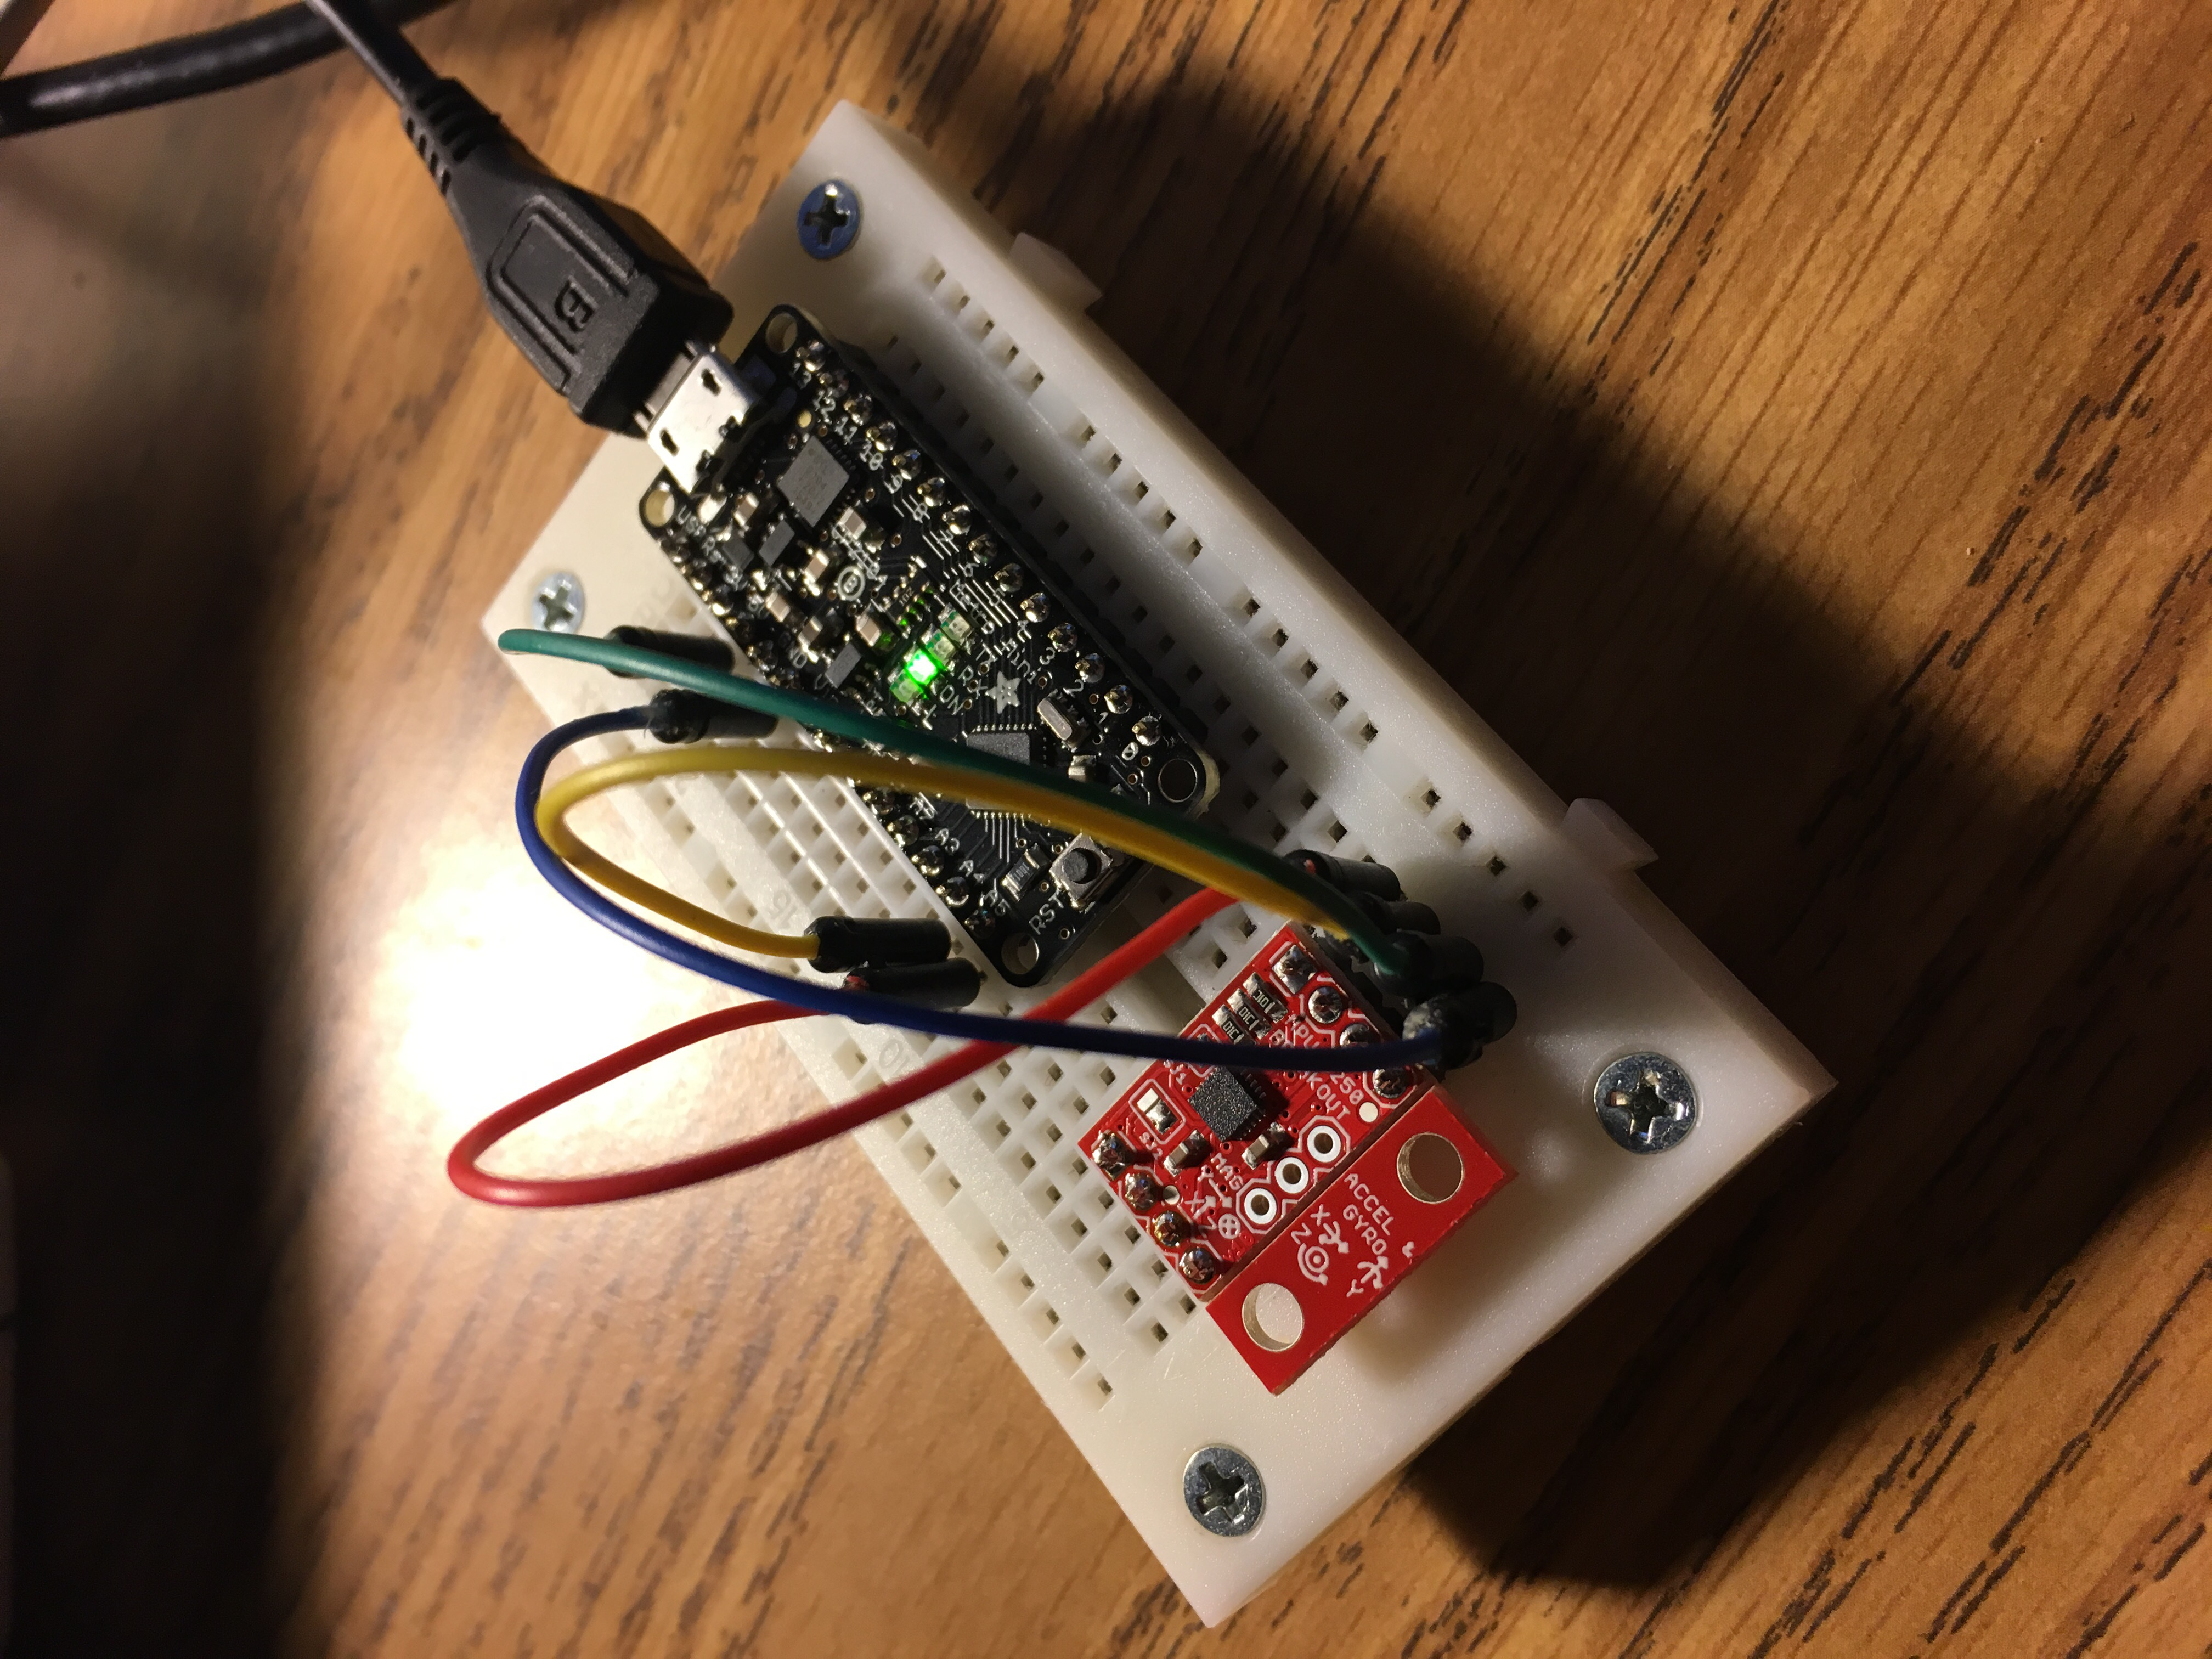
\includegraphics[width=0.5\textwidth ,height=0.5\textheight,keepaspectratio,angle=270,origin=c]{breadboard}
			    \label{fig:breadboard}
			\end{figure}



			\paragraph{Function Attribute}
			The entire system is constructed based on four major entities including a simulated aircraft object, a microcontroller, a HUD IMU and an aircraft IMU. In addition, an output display is necessary in this demonstration system for testing purpose but it is not part of the original system, that means this display is used for simulating the real HUD output on an aircraft. Respectively, these two IMUs in this demonstration system represent and simulate the functionalities for the real IMU component mounted on a head-up display of an aircraft and the aircraft body itself. Within this demonstration system, both IMUs may consist of one or more \textit{MPU-9250} (e.g., accelerometers). The simulated aircraft object provides motion input to the IMU sensors this object can be any kinds of vehicle or drone that is able to provide physical motion.\\


			\paragraph{Experiment Design for IMU Error Measurement}
			It is vital to know the actual error of all IMU sensors before using the data into the algorithm. A method to precisely measure the error is to compare a known inclined angle with the calculated angle from two sensor output results (before and after incline).

			\begin{figure}
				\centering
			 		\caption{Mechanical Angle Adjuster}
			      	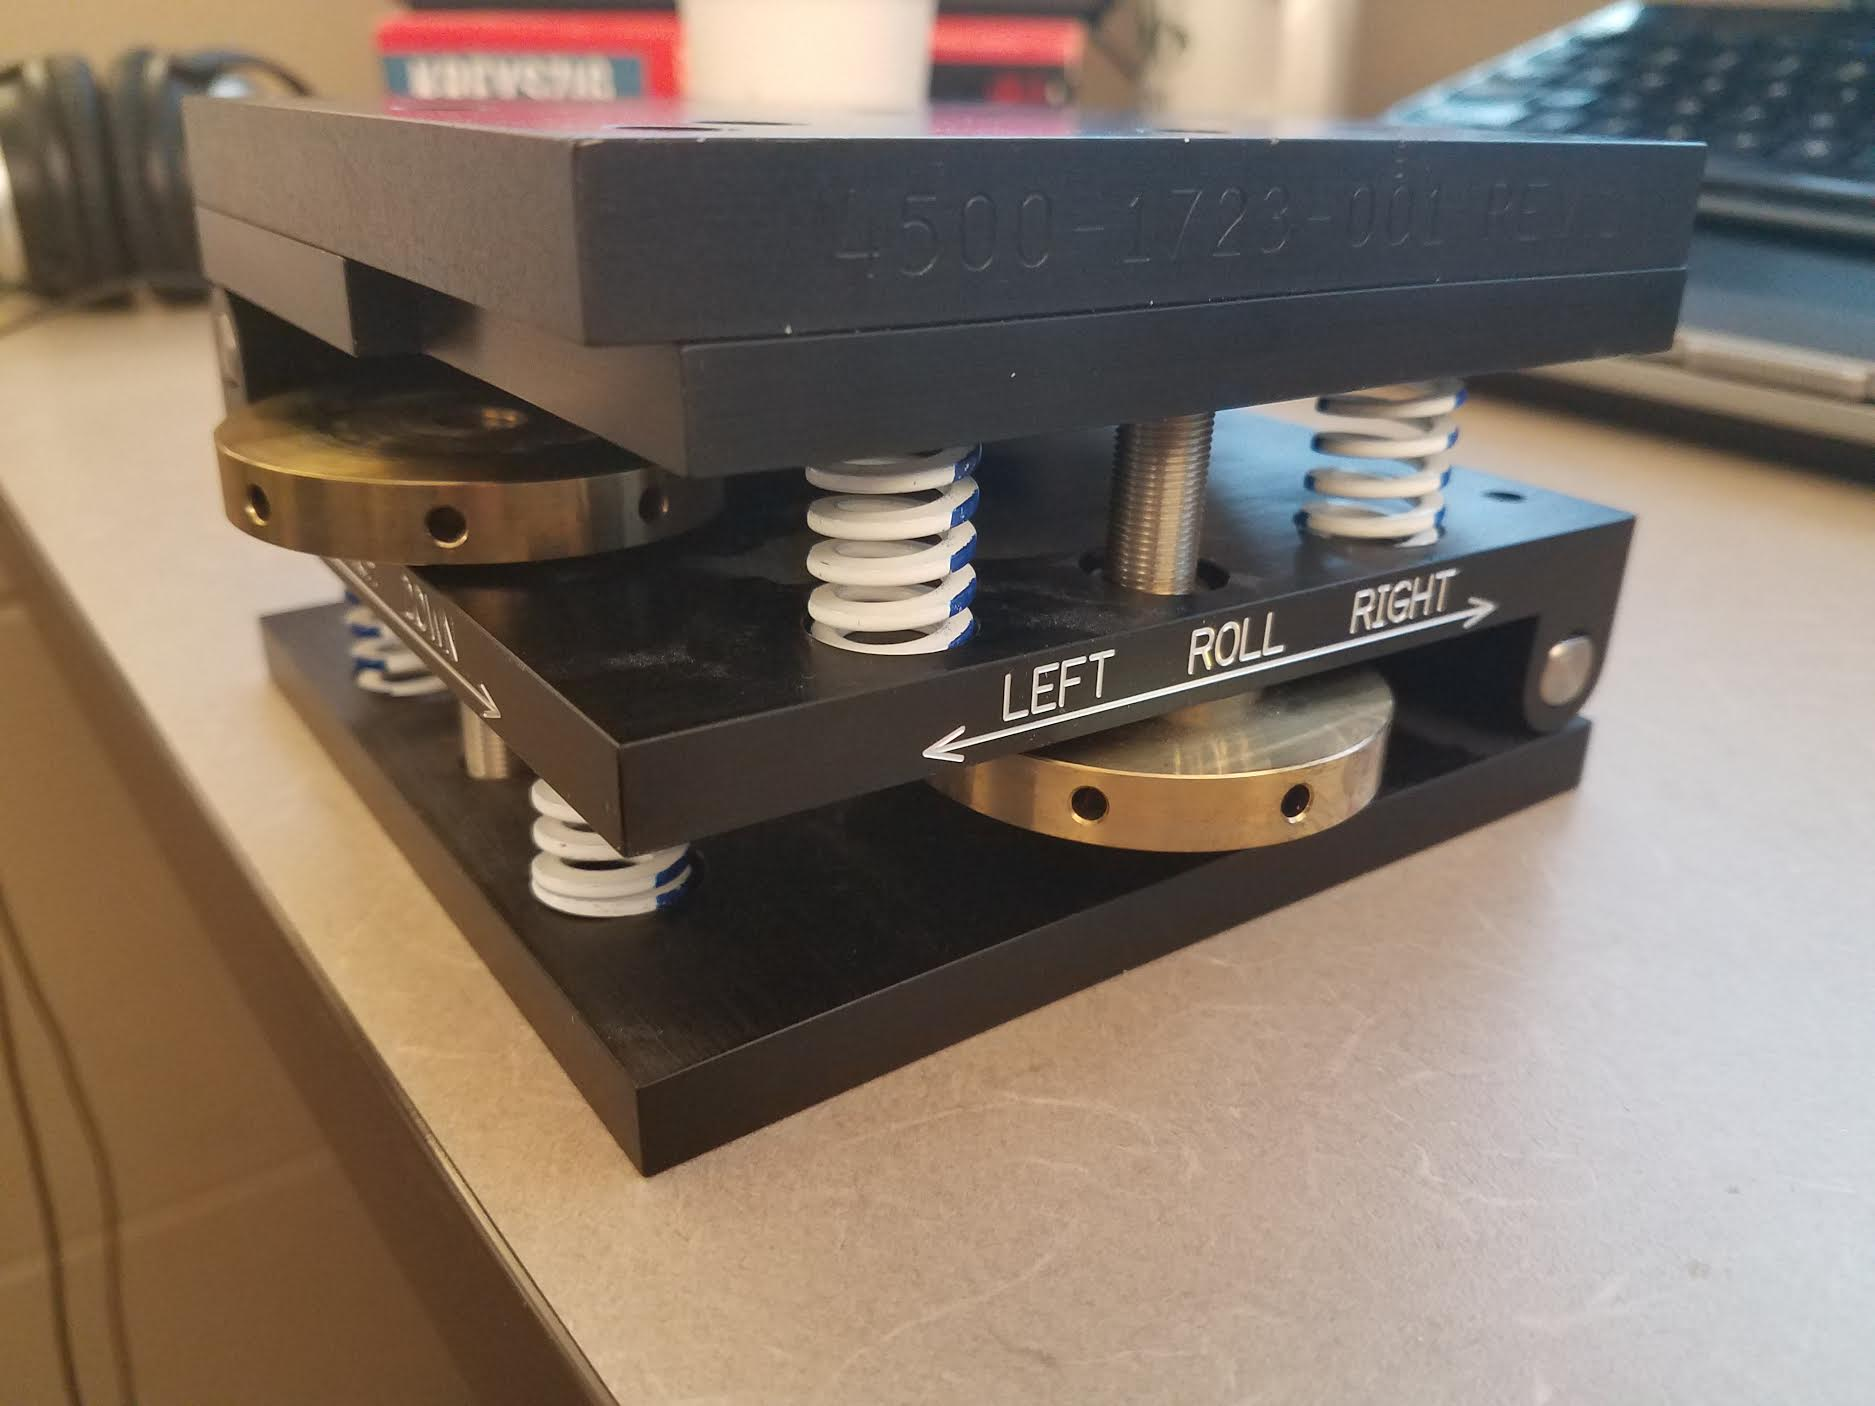
\includegraphics[width=0.5\textwidth,height=0.5\textheight,keepaspectratio]{widget}
			    \label{fig:widget}
			\end{figure}

			The experiment will be using a laser pointer and a mechanical angle adjuster as figure ~\ref{fig:widget} for assistant tool. A mechanical angle adjuster allows to be manually set for getting a certain degree of angle for simulating yaw, pitch and roll, that will be able to provide a stable motion for the IMU as well as error measurement. A laser pointer is also necessary, that a laser is for constructing a triangle by using the initial distance between the laser pointer and the wall (a), alternative distance between the laser pointer and wall, as well as the distance between two spotlight (b), refer figure~\ref{fig:draft}:

			\begin{figure}
				\centering
			 		\caption{Draft graph of error measurement experiment}
			      	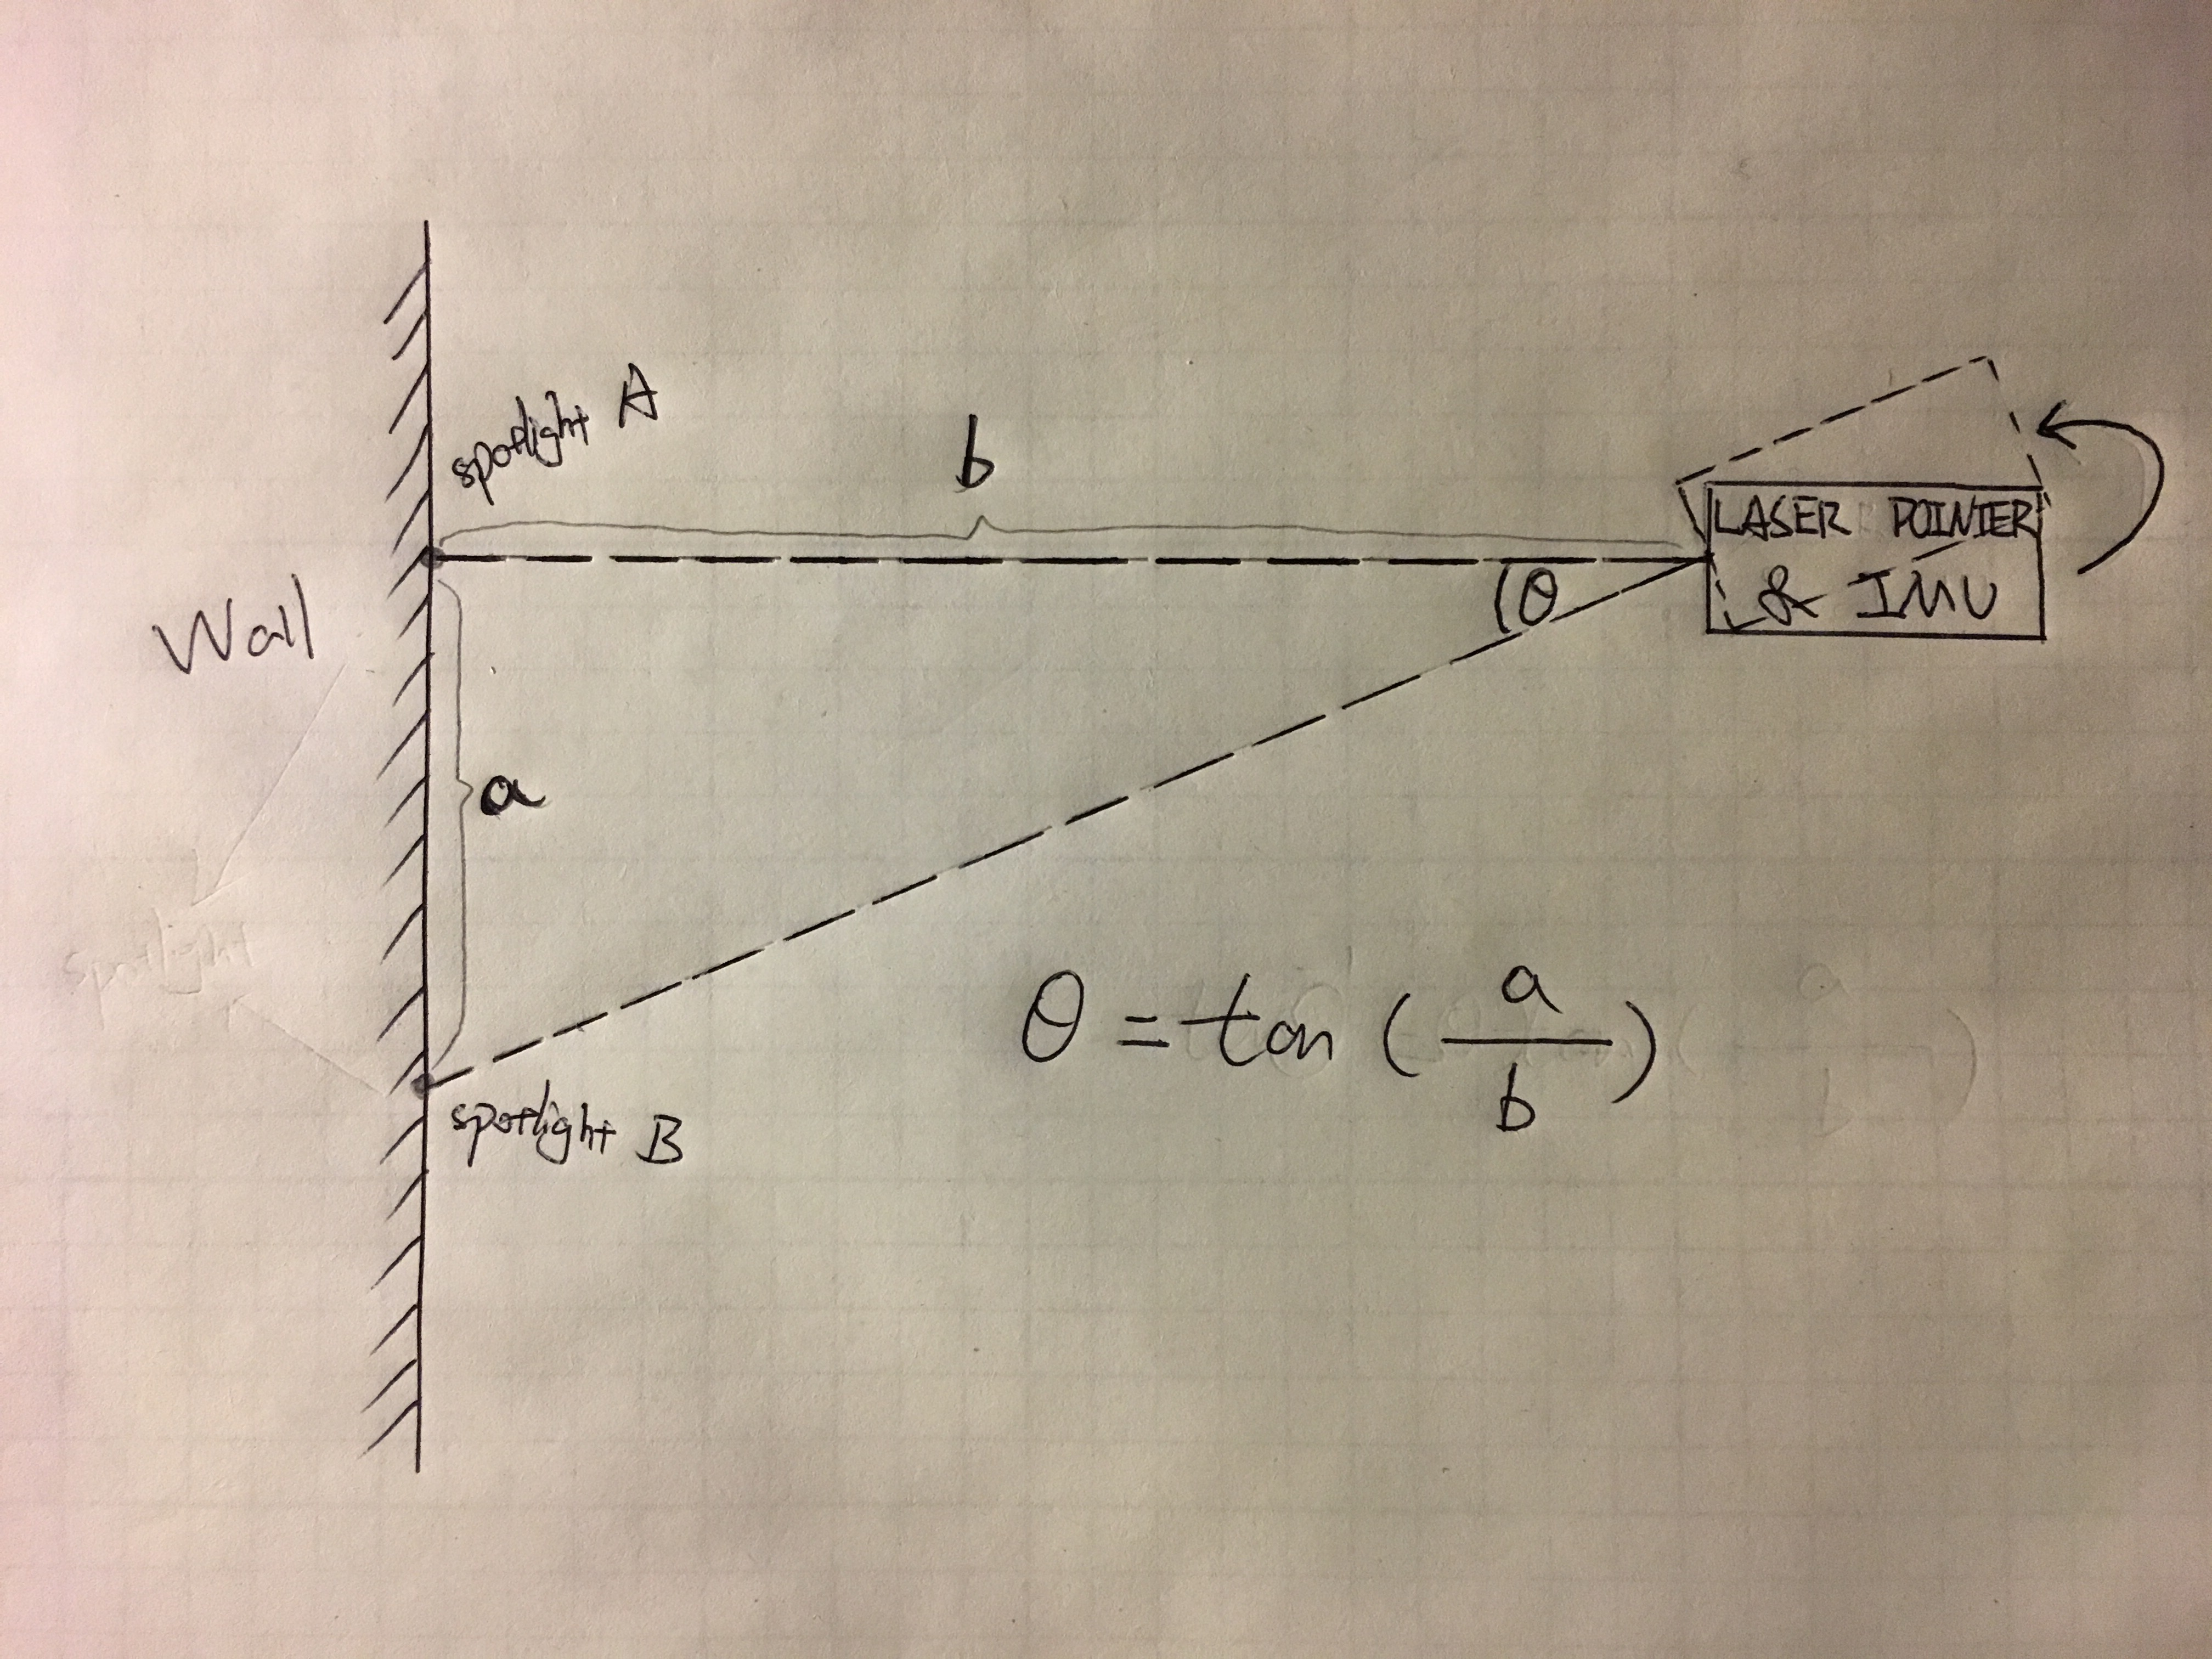
\includegraphics[width=\textwidth,height=\textheight,keepaspectratio]{draft}
			    \label{fig:draft}
			\end{figure}

			Theta represents the angle between adjusting the angle, and by measuring the distance value of “a” and “b”, theta can be calculated by applying trigonometric function. Assume theta is the actual precise angle (in radian), the error of the IMU sensor can be measured by comparing the actual precise angle with the output data from the IMU.

		\begin{figure}
			\centering
		 		\caption{Data Flow between Hardware Components}
		      	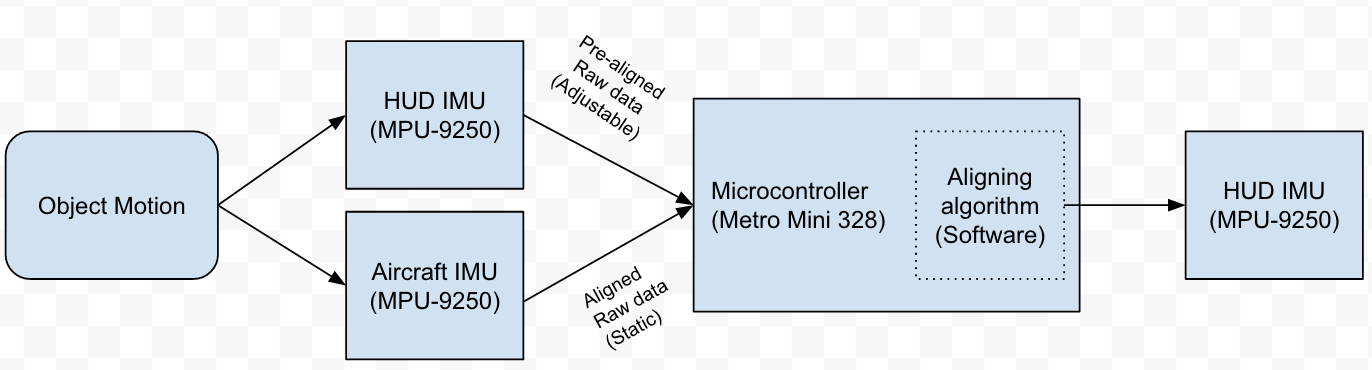
\includegraphics[width=\textwidth,height=\textheight,keepaspectratio]{composition1}
		    \label{fig:composition1}
		\end{figure}

%=======================================================================================
\section{Dependency View}
	\subsection{Dependency Design}
	This section will cover the interconnection of hardware and software throughout the system. This section is intended to summarize and explain all the necessary components in terms of their dependencies.\\

		\subsubsection{Design Concern}
		All components must have clearly defined relationships. All components within the system should be included in the dependency design, refer Figure~\ref{fig:dependency1} UML diagram for more detail.\\

		\subsubsection{Design Elements}
		\begin{itemize}
			\item HUD IMU: \textit{MPU-9250}.
			\item HUD IMU DMP: Provides on board filtering and 9-axis to quaternion conversion.
			\item Aircraft IMU: \textit{MPU-9250}.
			\item Aircraft IMU DMP: Provides on board filtering and 9-axis to quaternion conversion.
			\item Microcontroller: \textit{Metro Mini 328} .
			\item Offset Algorithm: Takes input from both IMU’s through the microcontroller and returns the offset between each other.
			\item Statistical Analysis Algorithm for Initial Alignment Offset: Takes multiple offset inputs until a valid initial offset can be returned.
			\item Statistical Analysis Algorithm for Dynamic Alignment Offset: Takes multiple offset inputs until a valid dynamic offset can be returned.
			\item Initial Offset: The value found that represents the initial alignment offset.
			\item Dynamic Offset: The value found that represents the dynamic alignment offset.
			\item HUD: Graphical output by a computer software (for demonstration system only).\\
		\end{itemize}

		\subsubsection{Dependency Attributes}
		See Figure~\ref{fig:dependency1}.\\

		\begin{figure}
			\centering
		 		\caption{Dependency UML Diagram}			%caption 
		      	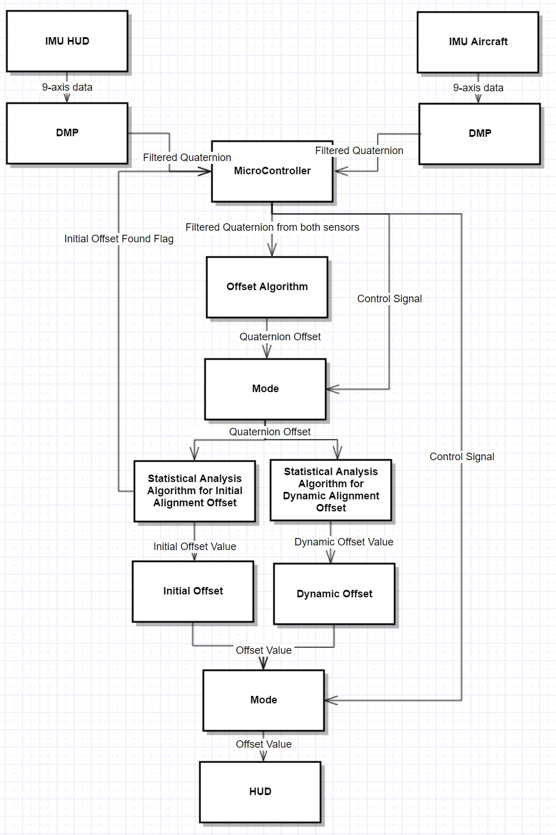
\includegraphics[width=\textwidth,height=\textheight,keepaspectratio]{dependency1}
		    \label{fig:dependency1}
		\end{figure}

		\subsubsection{Design Rationale}
		An overall view of the system is required to understand how each component fits into the system in relation to other components. By providing the dependency design, faults within the system can be determined by analyzing their specific scopes and connections. The dependency view will be used to determine the prioritization for component development to ensure that components are being developed by time of need to avoid blocking.

%=======================================================================================

\section{Interface View}
	\subsection{Software User Interface Design}
	This section will cover the specification of the software user interface portion for this project. This section is intended to guide the software development team to interact correctly with the software user interface.\\

		\subsubsection{Design Concerns}
		The goal of this project is to have a demonstration system that can be used by Rockwell Collins HUD system engineers to determine the availability of having an additional MEMS IRU in the new HUD alignment system. Graphical user interface will be crucial for our project presentation and demonstration system. The algorithm from our project will output a raw alignment data and it will be hard to understand the output without the help of graphical user interface. The graphical user interface will put context to the data and present the symbology of the alignment data output. A gauge icon is used to define the HUD symbology. The graphical user interface is created in Visual Studio IDE and ready to be connected to its Arduino program counterparts.\\

		\subsubsection{Design Elements}
		This section will cover the interface attributes that defines each functionality on the display and a paper prototype as Figure~\ref{fig:interface1}.

			\paragraph{Interface Attributes}
			\begin{itemize}
				\item \textit{Heading:} Display the direction of where the aircraft is pointing  
				\item \textit{Bank Angle:} Display the vertical elevation angle of the aircraft
				\item \textit{Pitch Angle:}  Display the angle between the aircraft and the horizon. Pitch angle shows the horizontal elevation angle of the aircraft 
				\item \textit{Credible Interval:} Display the degree of certainty of the alignment offset 
				\item \textit{Alignment Offset:} Display the calculated alignment offset detected by the algorithm 
				\item \textit{Original Data:} Display the original alignment data from the sensors 
				\item \textit{Aligned Data:} Display the calculated alignment data from the algorithm 
			\end{itemize}

			\begin{figure}[h]
				\centering
			 		\caption{The HUD Simulator}			%caption 
			      	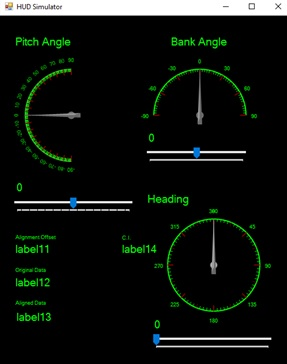
\includegraphics[scale=1]{interface1}
			    \label{fig:interface1}
			\end{figure}

		\subsubsection{Design Rationale}
		An important piece of this project is the dynamic alignment algorithm and our clients encouraged us to spend most our time in developing and refining the dynamic alignment algorithm. Learning that Rockwell Collins use a sophisticated software to generate their HUD display, using a full HUD display will also be out of scope for this project. We want to create a graphical user interface that is simple and serve its purpose as a medium for the user to understand the data being generated by the algorithm. We create this graphical user interface with Visual Studio Toolkit. The built in visual studio graphical user interface toolkit will help us to arrange the HUD symbology representation to its designated place and also display the appropriate data to the screen. We use a gauge to represent the HUD symbology. This user interface might not look like a flight simulator HUD, but it still serves its purpose. We also use 0 – 360 scale as the heading, where 0/360 is north, 90 is east, 180 is south, and 270 is west. 
		
	\subsection{Physical User Interface Design}
	This section will cover the specification of the physical user interface portion for this project. This section is intended to guide the software development team to interact correctly with the physical user interface in the demonstration system.\\

		\subsubsection{Design Concern}
		The goal of this project is to have a demonstration system that can be used by Rockwell Collins HUD system engineers to determine the availability of having an additional MEMS IRU in the new HUD alignment system. The user of this product will be able to directly interact with the physical user interface of this product. The physical user interface is the most interactive piece of this product. Refer to Figure~\ref{fig:interface2} The user will have the ability to adjust the precision adjustable wedge to simulate the HUD offset during flight. The user will also have the ability to move the board to simulate the airplane’s movement. This physical user interface settings is arranged to simulate the flight environment. Rockwell Collins will help us in creating the board with the precision adjustable wedge in it.\\

		\subsubsection{Design Elements}
		\paragraph{Interface Attributes}
			\begin{itemize}
				\item Board: A platform that can be moved to simulate the airplane movement 
				\item Precision adjustable wedge: An adjustable platform that can be moved to simulate the HUD alignment offset after initialization  
				\item “HUD” IMU sensors: The sensors that act as the HUD IMU 
				\item “Aircraft” IMU sensors: The sensors that act as the precisely aligned aircraft IMU.\\
			\end{itemize}

			\begin{figure}
				\centering
			 		\caption{Physical User Interface Design \cite{IMU-figure}}			%caption 
			      	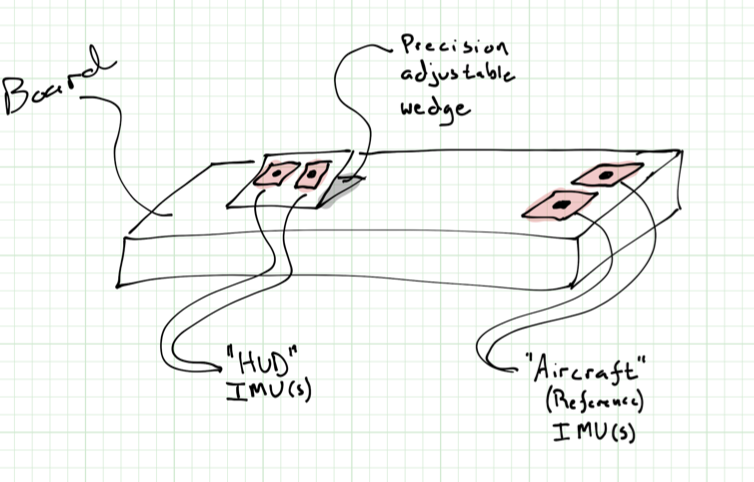
\includegraphics[scale=1]{interface2}
			    \label{fig:interface2}
			\end{figure}

		\subsubsection{Design Rationale}
		The physical user interface is a crucial piece of this project. This project algorithm is heavily based on the alignment and the set-up of our physical user interface. The physical user interface is an important part of our demonstration system. Our physical user interface is the most interactive piece of this product. Different than the software user interface, the user will be able to directly interact with our physical user interface. Our clients come up with the design for the physical user interface. We think that this is a great set-up to start our project. Since the wedge can be pre-aligned and adjusted, it eliminates some of our burden to find out the delta angle of the sensors. The precision adjustable wedge will also make our demonstration system more user friendly since it can be adjusted without requiring any additional tools. 

%=======================================================================================

\section{Interaction View}
	\subsubsection{Hardware Communication Design}
	This section will describe the communication methods between hardware components within the entire system. This section is intended to list out and describe how each hardware component talks with others including communication protocols and connecting methods.\\

	\subsubsection{Design Concerns}
	There are two necessary communications/connections for one input-output cycle, one is between the IMU and the microcontroller, the other is between the microcontroller and output display. Refer to the Technology Review for this project, there are three options for choosing the communication protocols between the IMU and the microcontroller: \textit{I2C}, \textit{SPI} and \textit{UART}. Based on our project design, \textit{I2C} protocol is the prior consideration for communicating between IMU and the microcontroller since \textit{Metro Mini 328} has limited pin numbers and \textit{I2C} only takes two pins (\textit{SDA} and \textit{SCL}) for wiring connection and \textit{I2C} provide fair transmission speed. In addition, USB is the appropriate communication method between the microcontroller and output display (computer) since \textit{Metro Mini 328} provides direct USB port and the makes the implementation simple and fast.\\ 

	\subsubsection{Design Elements}
		\paragraph{\textit{I2C} Protocol}
		One \textit{I2C} device (IMU) takes totally 4 pins to connect with a master board (microcontroller), besides VDD and GND pins, there are \textit{SDA} and \textit{SCL} which represent "serial data" and "serial clock" respectively. Both SDA and SCL are bi-direction wires, that means they can transfer sensor data to the master board, as well as transferring command data from the master board. The data rate has to be chosen between 100 kbps, 400 kbps and 3.4 Mbps, respectively called standard mode, fast mode and high speed mode. Some I²C variants include 10 kbps (low speed mode) and 1 Mbps (fast mode +) as valid speeds \cite{i2c-2}.

		In this system, there are more than one IMU sensors (\textit{MPU-9250}) needed to be working together in order to retrieve a higher accuracy data output. Hence, we choose to use \textit{I2C} protocol since it allows multi-devices communication. Additional devices are also known as the slave devices, referring to Figure~\ref{fig:interaction1}, \textit{I2C} allows \textit{I2C} device \#1 and \#2 (these represent \textit{MPU-9250} in this project) to communicate with each other by just using one SDA and one SCL wire (besides of VCC and GND), there is no need for extra “chip select pins” like SPI protocol for extra devices.\\

		\begin{figure}
			\centering
		 		\caption{\textit{I2C} Connection between Slave Devices}			
		      	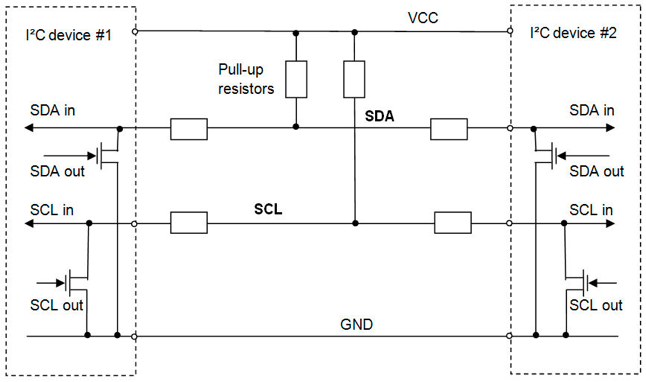
\includegraphics[width=\textwidth,height=\textheight,keepaspectratio]{interaction1}
		    \label{fig:interaction1}
		\end{figure}

		\paragraph{Universal Serial Bus}
		\textit{Metro Mini 328} uses Universal Serial Bus (USB) connection as default communication method between microcontroller and output display (computer). Specifically, \textit{Metro Mini 328} provides a Micro-USB (B) port, the implementation of this connection is simple and fast.\\

	\subsubsection{Design Constraints}
	Either the Aircraft or HUD IMU consists of multiple \textit{MPU-9250} sensors units, they can be put parallel together and act as an entity. See as Figure~\ref{fig:interaction2}, both IMUs will be connected to an \textit{I2C} Multiplexer separately by \textit{I2C} protocol. An \textit{I2C}  multiplexer allows the microcontroller to select the particular IMU unit based on the address that the \textit{I2C} Multiplexer assign to that IMU, so that we can easily split two groups of data (from HUD and Aircraft IMU) for the software program. Finally, an output display will retrieve a finalized aligned data from the microcontroller and allows for testing.

	\begin{figure}
		\centering
	 		\caption{Communcation Method between System Hardware Components \cite{i2c-2}}			
	      	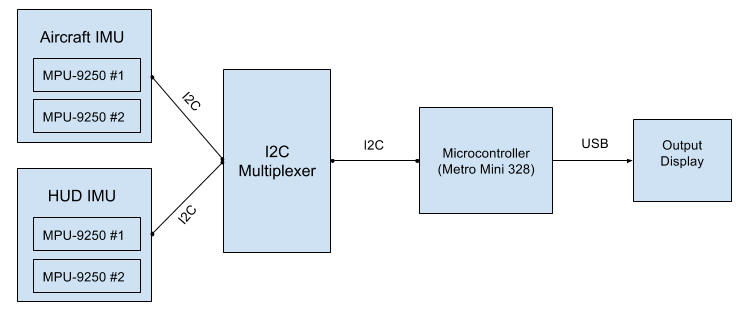
\includegraphics[width=\textwidth,height=\textheight,keepaspectratio]{interaction2}
	    \label{fig:interaction2}
	\end{figure}



\section{Algorithm View}
	\subsection{Statistical Analysis Method for Initial Alignment Offset Design}
	This section will cover the specification of the statistical analysis method for initial alignment of this project. This section is intended to guide the software development team to develop a suitable algorithm. This algorithm is intended to calculate the proper initial alignment data from the sensors under an acceptable degree of certainty.\\  

		\subsubsection{Design Concerns}
		Our primary goal is to find the initial alignment offset. Using a statistical analysis method is desired to ensure an accurate result. This algorithm requires the input of both sensors taken at the same time. A series of inputs will be received by this algorithm until the offset has been found to be within one milliradian of accuracy.\\

		\subsubsection{Design Elements}
		This section will cover the algorithm attributes that defines each functionality of the statistical analysis method for initial alignment offset

			\paragraph{Processing Attributes}
			\begin{itemize}
				\item \textit{Assumption:} The offset algorithm will calculate the correct alignment offset  value 
				\item \textit{Prerequisite:} Both sensors must be transmitting data that corresponds to the same time values.
				\item \textit{Input:} A series of sensor input values.
				\item \textit{Output:} An alignment offset value that best represent the alignment error under an acceptable credible interval 
				\item \textit{Acceptable Range:} 95\% credible interval 
				\item \textit{Acceptable Accuracy:} unit milliradian\\
			\end{itemize}

		\subsubsection{Design Rationale}
		Confidence interval, credible interval, and tolerance interval are three possible options of statistical analysis method that we can use to gain credibility of our alignment data. The confidence interval will give us the frequency of the true value output being generated by the algorithm over a time period. However, until the time of calculation, we are not sure what kind of value that we will get from the algorithm. Hence, leaving us with no parameter to work on confidence interval. The tolerance interval will give us the spread of error in alignment data being generated by the algorithm. This statistical method can be useful for us to further refine our algorithm. Credible interval will give us the credibility to state the certainty of a true value within an interval of data. This method will give us the true value that might be a great representation of our alignment data. We think that credible interval method fits the most with our project. Thus, this makes us decide to do credible interval for our statistical analysis method.

	\subsection{Statistical Analysis Method For Dynamic Offset Design}
	This section will cover the implementation details of the statistical analysis method for the offset error of this project. This section is intended to guide software developer to develop a suitable algorithm. This algorithm is intended to calculate the proper offset error value under an acceptable degree of certainty.\\ 

		\subsubsection{Design Concerns}
		The goal of using a statistical analysis method is to find the credibility of the output that we get from the algorithm. This algorithm will get its input from the offset algorithm. Then, the alignment error data that we get from the offset algorithm will be processed by this algorithm to find the credible interval for a range of offset error values. This algorithm will find the credible interval of the alignment error data and decide which value is best represent the alignment error for that instance. Referring to Figure~\ref{fig:algorithm1} for specific process details.\\

		\subsubsection{Design Elements}
		Elements include assumption, prerequisite, expected input, expected output of this algorithm. This section will also cover the method and formula that we will be using to create this algorithm.

			\paragraph{Processing Attributes}
				\begin{itemize}
					\item \textit{Assumption:} The offset algorithm will calculate the correct alignment error value 
					\item \textit{Prerequisite:} An alignment error value produced by the offset algorithm 
					\item \textit{Input:} A range of alignment error values 
					\item \textit{Output:} An alignment error value that best represent the alignment error under an acceptable credible interval
					\item \textit{Acceptable Range:} 95\% credible interval 
					\item \textit{Acceptable Accuracy:} unit milliradian\\
				\end{itemize}

		\begin{figure}
			\centering
		 		\caption{Statistical Analysis Algorithm Process}			
		      	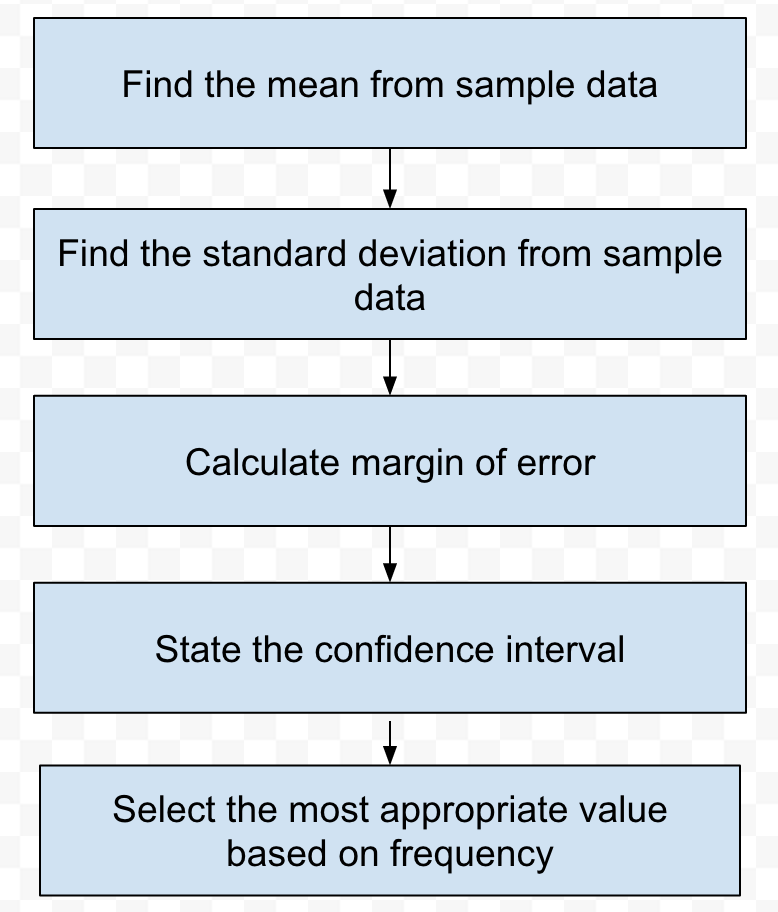
\includegraphics[scale=0.5]{algorithm1}
		    \label{fig:algorithm1}
		\end{figure}

		\subsubsection{Design Rationale}
		Confidence interval, credible interval, and tolerance interval are three possible options of statistical analysis method that we can use to gain credibility of our alignment data. The confidence interval will give us the frequency of the true value output being generated by the algorithm over a time period. However, until the time of calculation, we are not sure what kind of value that we will get from the algorithm. Hence, leaving us with no parameter to work on confidence interval. The tolerance interval will give us the spread of error in alignment data being generated by the algorithm. This statistical method can be useful for us to further refine our algorithm. Credible interval will give us the credibility to state the certainty of a true value within an interval of data. This method will give us the true value that might be a great representation of our alignment data. We think that credible interval method fits the most with our project. Thus, this makes us decide to do credible interval for our statistical analysis method.\\

	\subsection{Offset Algorithm Design}
	This section will cover the implementation details of the offset algorithm for this project. This section is intended to guide software developer to develop a suitable algorithm. This algorithm is intended to calculate the proper offset between two quaternion inputs.\\

		\subsubsection{Design Concerns}
		The resulting output must be the quaternion offset of two quaternion inputs. The algorithm will first take the input of the first input. The next step will be to multiply both inputs against each other. The resulting multiplication will be the desired output.\\

		\subsubsection{Design Elements}
			\paragraph{Processing Attributes}
					\begin{itemize}
						\item Quaternion input A: The first of two quaternion inputs
						\item Quaternion input B: The second of two quaternion inputs
						\item Quaternion output offset: The resulting offset with the form of quaternion\\
					\end{itemize}

		\subsubsection{Design Rationale}
		The design requires an offset in terms of a quaternion output in order to be used within the rest of the system. 

\section{Conclusion}
This design document has covered six main design views from the perspective of hardware and software, each view contains specific design viewpoints as well as relevant detailed explanations. This document would help and provide necessary plan information for our project implementation in terms of hardware set-up, algorithm design, testing and debugging. More importantly, this design document allows us to think thoroughly over the entire implementation process, and helps us move forward with in the development of our solutions to the problem.
































